\documentclass[aps,prl,twocolumn,showpacs, superscriptaddress,floatfix, 10pt]{revtex4-1} 
\usepackage{amsmath}
\usepackage{amssymb}
\usepackage{graphicx} 
\usepackage{color}
\usepackage{float}


\begin{document}

\section*{Supplemental material}

\setcounter{figure}{0}
\makeatletter 
\renewcommand{\thefigure}{S\@arabic\c@figure}
\makeatother

\begin{figure}[H] 
	\centering
	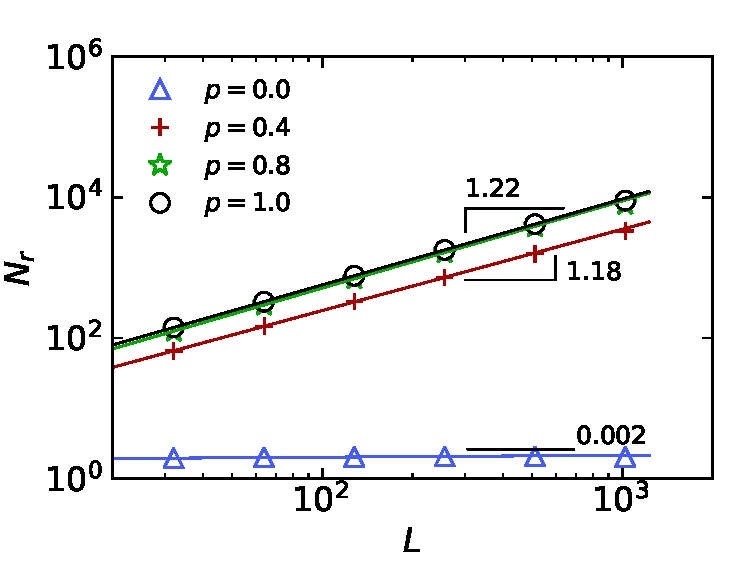
\includegraphics[width=0.85\columnwidth]{figS1} 
\caption{Logarithmic dependence of the total number of removed links $N_r$
on the linear size of the lattice $L$, for different values of the fraction
$p$ of unidirectional links. The symbols correspond to averages over $100$
thousand network realizations with sizes $L=16$, $32$, $64$, $512$, and
$1024$ and strong disorder in their traveling times ($\beta=400$). The
results for $p=0.4$ and $0.8$ are consistent with the scaling, $N_r\sim
L^D_f$, with $D_{f}=1.22\pm 0.01$ obtained for $p=0$, namely, fully
bidirectional lattices~[16].  For a completely unidirectional lattice,
$p=1$, we find that $N_r\sim L^{D_f}$, with $D_f=0.002\pm 0.004$. The error
bars are smaller than the symbols.} 
\end{figure}
%~\label{fig::strong.disorder}


\begin{figure}[H]
	\centering
	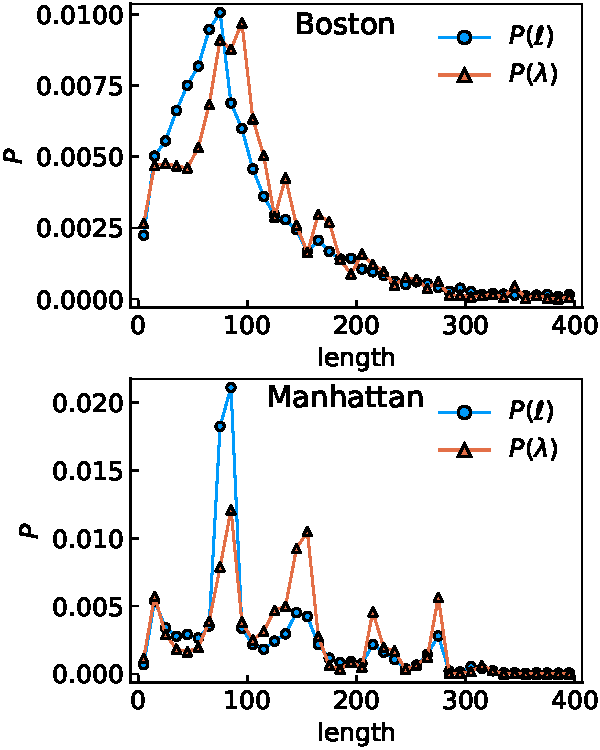
\includegraphics[width=0.8\columnwidth]{figS2} 
\caption{ Comparison between distributions of the lengths $\ell$ of all
road segments, and the lengths $\lambda$ of those among all road segments
that have been removed  during the OPC process applied to Boston (top) and
Manhattan (bottom).}
\end{figure}
%~\label{fig::distributions.ell.lambda}

\begin{figure}[H]
	\centering
	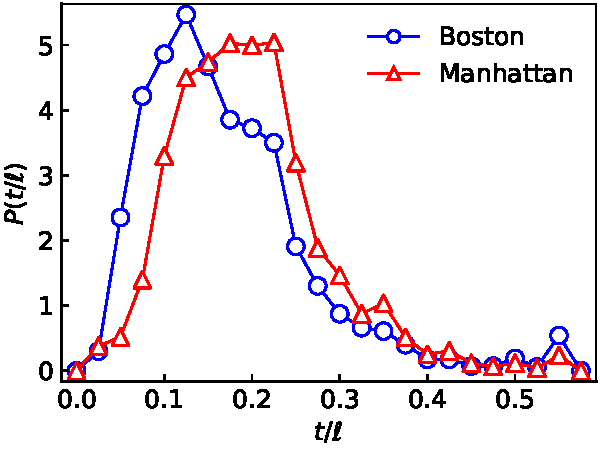
\includegraphics[width=0.8\columnwidth]{figS3} 
\caption{Distributions of ratios $t/\ell$ for all road segments of Boston
(circles) and Manhattan (triangles).}
\end{figure}
%~\label{fig::distributions.t.ell}

\begin{figure}[H]
\centering
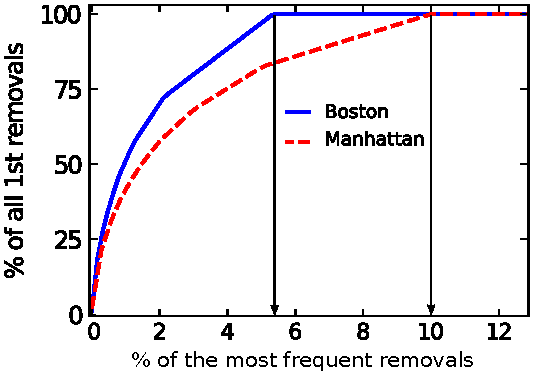
\includegraphics[width=0.85\columnwidth]{figS4} 
\caption{Cumulative dependence of the percentage of all first removals
during the OPC process on the fraction of the most frequent ones. The
vertical solid lines indicate that the first removals correspond to $5.4\%$
of all road segments in the case of Boston, while $10.0\%$ is the
percentage required for Manhattan.}
\end{figure}
%~\label{fig::cummutative.fraction.removed}

\end{document}

